% Dans l'introduction, on présente le problème étudié et les buts
% poursuivis. L'introduction permet de faire connaître le cadre de la
% recherche et d'en préciser le domaine d'application. Elle fournit
% les précisions nécessaires en ce qui concerne le contexte de
% réalisation de la recherche, l'approche envisagée, l'évolution de
% la réalisation. En fait, l'introduction présente au lecteur ce
% qu'il doit savoir pour comprendre la recherche et en connaître la
% portée.
\Chapter{INTRODUCTION}\label{sec:Introduction}  % 10-12 lignes pour introduire le sujet.
%Texte en \emph{italique}, \textsc{petites majuscules}, mot \mbox{insécable}.\\
%Texte \ul{souligné}, \hl{surligné}, \textbf{gras}.\\
%Texte entre ``guillemets''.\\
%Police \texttt{monospace}.\\
%Un mot courant en réseautique mobile: n\oe{}ud\footnote{Note de bas de page.}.\\
%L'objet RSVP \texttt{SENDER\_TEMPLATE}.\\
%%Nom d'un auteur: \citeauthor{RFC_IPv4}.\\
%Une architecture 32~bits.\\
%%%
%%%  CONCEPTS DE BASE / BASIC CONCEPTS
%%

Conduire ses travaux de recherche sur la vision par ordinateur quand celle-ci a pour objectif le diagnostic de la vision humaine: voilà une curieuse conjonction qui ne peut que satisfaire l'intérêt de la chercheuse ou du chercheur qui s'y atèle. Donner -métaphoriquement- la vue à un algorithme, l'entraîner à déceler ce que l'\oeil{} du médecin sait détecter, démocratiser ainsi l'accès aux soins: voilà fondamentalement le cœur du projet qui motive la communauté scientifique affairée à la détection des maladies rétiniennes. Cette volonté de créer une assistance médicale se pare parfois d'un second objectif: faire émerger, grâce à la puissance computationnelle des algorithmes, des nouveaux modes de compréhension des maladies, de leur pathogenèse et de leur mécanisme de progression et ainsi accroître le corpus des connaissances scientifiques. Ce qui rend cette recherche si passionnante dans un cas comme dans l'autre, c'est son positionnement à la confluence de domaines aussi distincts que les mathématiques, l'informatique et la biologie. \\
Les perspectives à moyen voire court terme ne peuvent que motiver davantage la recherche dans ce domaine. En effet, tous usages confondus, les algorithmes \og apprenant \fg ont récemment fait preuves de progrès spectaculaires. Or, les principales pathologies rétiniennes sont en forte augmentation à travers le monde (conséquence entre autres du vieillissement des populations). Fort heureusement les progrès technologiques (comme la numérisation) ont rendu possible la massification de l'imagerie rétinienne. Face à cette double conjonction, l'automatisation de certains aspects du diagnostic est présentée comme une des briques manquantes des campagnes de dépistage à large échelle, voire apparaît de plus en plus comme une nécessité impérieuse. Ce constat est clairement partagé dans le milieu académique, en témoigne l'impressionnante quantité de production scientifique publiée. À ce propos, parler d'effervescence relève de l'euphémisme; pour s'en convaincre il suffit de regarder la courbe du nombre d'articles liés à la fois à l'apprentissage machine et à la rétine publiés ces dix dernières années (figure \ref{fig:articlesPublies}): la croissance est exponentielle et ne manifeste pour l'instant aucun signe de ralentissement.
\begin{figure}[!ht]
	\centering
	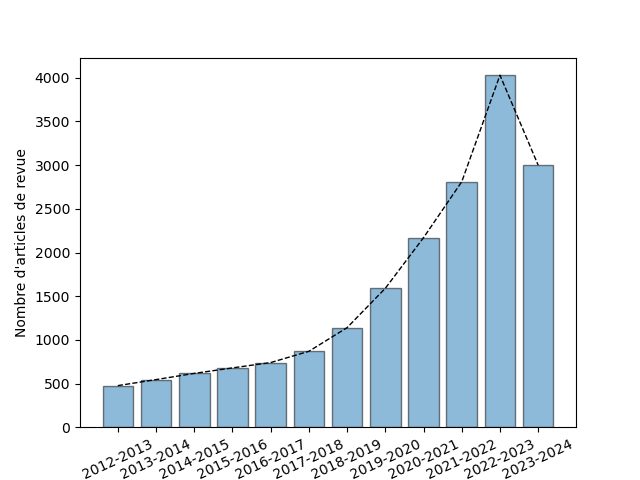
\includegraphics[width=0.8\textwidth]{paper_published}
	\caption{Nombre d'articles de revues recensés sur \textit{Google Scholar} avec les mots clés \og \textit{machine learning, retina} \fg.}
	\label{fig:articlesPublies}
\end{figure}


Cet engouement est en réalité fort logique car la rétine est un tissu particulièrement propice à la recherche informatique. En effet, l'imagerie rétinienne est (en général) non invasive et relativement peu onéreuse. Cela facilite la collecte et le partage des données à large échelle et donc la communion des efforts de recherche. Plus généralement, un bon nombre de diagnostic de pathologies rétiniennes s'appuie sur la lecture et l'interprétation d'image: or la vision par ordinateurs s'est dotée de nombreux nouveaux outils puissants sur la dernière décennie. L'engouement autours de la détection automatique de pathologies rétiniennes était donc prévisible. 
Cependant, cette récente prolifération des savoirs ne signifie pas la résolution de tous les obstacles qui jalonnent le chemin entre le laboratoire où est conçu l'algorithme  et le chevet du patient. Deux problèmes, parmi d'autres, reviennent régulièrement:
\begin{itemize}
	\item Quelle garantie existe-t-il de l'efficacité d'un algorithme une fois celui-ci sorti de l'univers calibré du laboratoire et appliqué au monde clinique? Autrement dit, comment garantit-on ses performances? Cette question s'inscrit dans le contexte de la \textbf{généralisation}.
	\item Comment encourager l'acceptabilité clinique d'un dispositif automatique? Un algorithme peut-il obtenir la confiance du clinicien ou du patient, de son concepteur ou des autorités de santé? Ce questionnement est au c\oe{}ur de tout un pan de la recherche dédié à l'\textbf{interprétabilité} des modèles. 
\end{itemize}
C'est sous le prisme de ces deux notions que s'inscrit ce doctorat. Cette recherche a évolué au fil du temps et au gré des collaborations entre les équipes d'ophtalmologie et de recherche de l'hôpital Maisonneuve-Rosemont de Montréal et du laboratoire LIV4D de l'École Polytechnique. Bien que l'application clinique soit toujours en ligne de mire, nos travaux s'inscrivent résolument dans le champs de l'apprentissage machine et le développement de nouveaux concepts fondamentaux. Pour cette raison, nous n'avons pas cantonné nos expériences à une seule modalité d'imagerie ni à une maladie spécifique. Au contraire, quand cela était possible, nous avons pris le parti d'exploiter les plus grandes collections de données possibles pour éprouver nos propositions théoriques sur les deux thématiques de généralisation et d'interprétabilité. Ce n'est donc pas la conception et le développement d'un seul modèle très spécialisé que présente cette thèse, mais les questionnements théoriques et pratiques auxquels un tel modèle se doit de répondre. À ces questionnements et dans la lignée de la littérature, nous proposerons des hypothèses de réponses et leur vérification. Ainsi, traiter de plusieurs maladies et de multiples modalités nous permet d'élargir la portée de nos conclusions. La structuration de ce document suivra cette logique: bien qu'il existe un fil conducteur entre elles, nos contributions méthodologiques peuvent se lire indépendamment les unes des autres. Mais avant de les présenter, le reste de la présente introduction vise à fournir les éléments de contexte permettant de familiariser le lecteur aux notions traitées.


\section{Éléments de la problématique}  % environ 3 pages
\subsection{Contexte anatomique et clinique}

Pour saisir les différents composantes de notre problématique, il est important de s'appuyer sur le contexte dans lequel s'inscrit ce doctorat. La recherche sur l'imagerie médicale impose un certain nombre de contraintes spécifiques: 
\begin{itemize}
	\item L'interprétation d'une image ne peut se faire sans faire sans un minimum d'expertise sur la structure anatomique imagée. La collaboration avec les médecins est donc souvent indispensable, en particulier pour l'annotation des données qui ne peut se faire sans leur contribution. 
	\item Plus pragmatiquement, la collecte des données est en général plus ardue que sur d'autres domaines. Plusieurs facteurs l'expliquent: le respect du consentement éclairé du patient est impératif et l'approbation par comité éthique avant collecte rajoute des étapes protocolaires. Chaque acquisition est donc coûteuse en temps ou en moyens (pour le patient et les équipes médicales en charge).
\end{itemize}
À la différence peut-être d'autres applications du \textit{Big Data}, ces contraintes rendent chaque donnée individuelle très précieuse. Il est donc important pour quiconque la manipule -y compris le chercheur en informatique- de comprendre a minima les bases anatomiques de la structure imagée, les contraintes physiques liées à la modalité d'acquisition et la manifestation des pathologies qu'on souhaite pouvoir détecter. Cette section se consacre donc à détailler ces différents points.

\subsubsection{Structure de l'\oeil.}

L'\oeil{} transforme la lumière reçue en influx nerveux qui sont transmis au cerveau. Tout comme un appareil photographique ne peut être réduit à un simple capteur photonique, l'\oeil{} est constitué d'un ensemble sophistiqué de tissus venant guider la lumière vers la rétine. Dans son apparence externe et à l'\oeil{} nu, le globe oculaire se compose de la sclère (\og blanc de l'\oeil{}\fg{} ) et de la cornée. La sclère est une structure résistante, visant à protéger l'\oeil{} des dégâts mécaniques. Elle est recouverte (hormis sur sa partie antérieure) par la conjonctive, responsable de la production du mucus intégrant la composition du liquide lacrymal. Sur sa partie antérieure, la sclère est percée pour laisser place à la cornée. Il s'agit d'une membrane circulaire bombée et transparente constituée à 78\% d'eau. Les larmes produites par les glandes lacrymales viennent l'alimenter en permanence et sont réparties sur toute sa surface par le battement des paupières. Elle est la principale responsable de la focalisation des rayons lumineux pénétrant l'\oeil{}: à elle seule, elle assure près de 80\% de la réfraction. Derrière la cornée se trouve une ouverture, nommée pupille, fonctionnant comme un diaphragme. La largeur de la pupille, contrôlée par les muscles lisses de l'iris, permet d'adapter la quantité de lumière pénétrant l'\oeil{}. \\
Pour assurer une mise au point aussi bien sur des objets lointains que proches, la focalisation doit être dynamique. Cette dynamique est rendue possible grâce au cristallin, petit disque fibreux situé à l'arrière de la cornée. La tension du cristallin est contrôlée par le corps ciliaire, constitué d'un réseau de muscles (muscles ciliaires) et également responsable de la sécrétion de l'humeur aqueuse. L'ensemble cornée/cristallin joue le rôle de doublet optique dont la longueur focale est régulée par la tension appliquée au cristallin.
Derrière ce dernier se trouve le corps vitré, où circulent les rayons lumineux avant de converger vers la surface tapissant l'intérieur du globe oculaire. Cette dernière, appelée rétine, est responsable de la conversion électromagnétique du signal lumineux en impulsions nerveuses. 


\subsubsection{Anatomie  de la rétine}
\label{sec:AnatRetina}
La vision humaine est le résultat de l'interaction complexe entre la lumière et des photorecepteurs qui convertissent et envoient les signaux nerveux au cerveau. Le siège de cette interaction se trouve dans la rétine, tissu qui tapisse la surface interne de l'\oeil. Au cours de l'embryogènese, la rétine se développe depuis la cupule optique (tête du nerf optique), une excroissance issue du cerveau frontal \cite{willoughbyAnatomyPhysiologyHuman2010}. De cette tête de nerf optique émergera le réseau vasculaire chargé d'irriguer l'ensemble des couches de la rétine; il est compris d'artères, de veines et de micro-vaisseaux nommés capillaires rétiniens. En ce qui concerne les couches rétiniennes, elles se distinguent par le type de neurones qui les composent. Il en existe cinq classes majeures dans la rétine: les photorécepteurs, les cellules bipolaires, les cellules horizontales, les cellules amacrines et les cellules ganglionnaires. Sur des coupes histologiques, on peut en dénombrer un nombre plus important encore et observer précisément l'organisation en couches de ceux-ci.
Radialement (en suivant le chemin de la lumière  arrivant dans l'\oeil), ces couches rétiniennes superposées sont:
\begin{enumerate}
	\item La membrane limitante interne, composée des cellules de Müller.
	\item La couche des fibres nerveuses, c'est à dire les axones des cellules ganglionnaires. 
	\item La couche des cellules ganglionnaires, qui contient leurs noyaux.
	\item La couche plexiforme interne formée des cellules amacrines
	\item La couche nucléaire interne formée des cellules bipolaires
	\item La couche plexiforme externe formée des cellules horizontales
	\item La couche nucléaire externe, où se situent les photorécepteurs (cônes et bâtonnets).
	\item L'épithélium pigmentaire (ou RPE pour \textit{Retinal Pigment Epithelium}), par où se font les échanges nutritifs et apports sanguins entre la rétine et les structures plus profondes.
\end{enumerate}
Sous cette dernière couche se trouve un second tissu, appelé la choroïde. C'est par celle-ci, très vascularisée, que se fait la nutrition de l'iris et des photorécepteurs. Parmi ceux-ci, la distinction entre cônes et bâtonnets permet d'expliquer la vision en couleur et et la vision périphérique. Tout comme la plupart des vertébrés, l'être humain possède ces deux types de cellules, les bâtonnets étant près de vingt fois plus nombreux que les cônes (on compte entre 110 et 130 millions de bâtonnets pour environ 7 millions de cônes). 
Les cônes sont responsables de la perception de la couleur. Ils contiennent différents pigments réagissant respectivement à trois plages de longueurs d'onde en envoyant un influx nerveux au cerveau. Ces longueurs d'ondes correspondent à peu près au bleu, au vert et au jaune sur le spectre de la lumière. Les bâtonnets pour leur part ne disposent que d'un type de pigment, sensible aux longueurs d'onde proche du bleu; ils sont par conséquent incapable de distinguer les couleurs. En revanche, étant plus sensibles, ils restent actifs même en faible luminosité. Chez l'humain, près de 50\% des cônes sont situés au sein d'une structure centrale appelée macula, au centre de laquelle se trouve la fovéa, point central concentrant la majorité des cônes. 
\\
La macula est donc le point central de la vision. Il s'agit d'une région elliptique de \SI{1,5}{\milli\meter} de large pour \SI{1}{\milli\meter} de hauteur. Au niveau de la fovéola (centre de la fovéa), elle est très mince (\SI{130}{\micro\meter}). La région dépressionnaire de la fovéola est bordée par une structure en bourrelet nommée clivus, d'une épaisseur de \SI{410}{\micro\meter}. Ailleurs, l'épaisseur moyenne de la rétine varie entre \SI{180}{\micro\meter} à l'équateur et va en diminuant sur la périphérie (jusqu'à \SI{100}{\micro\meter}). Ces différentes structures sont visibles par des coupes histologiques ou in vivo par l'imagerie de \fundus{} et de la \ac{OCT}.
\\
Cette brève description de la rétine va nous permettre d'introduire les deux grandes pathologies pouvant l'affecter et les manifestions cliniques que celles-ci déclenchent. Mais auparavant, nous ouvrons une brève parenthèse sur les modalités permettant d'imager la rétine.

\subsubsection{Modalités d'acquisition de l'imagerie rétinienne}
La photoréception se faisant dans la rétine, celle-ci possède intrinsèquement une propriété particulièrement propice à l'imagerie: en effet, si les rayons lumineux se focalisent en son sein, il est possible de leur faire parcourir le chemin inverse pour reconstruire une image de celle-ci. L'observation de la rétine peut donc se faire de manière non invasive (c'est-à-dire sans injection d'agents de contraste, sans radiation ni opération chirurgicale). \\
De nombreuses modalités ont été développées pour la visualiser. Nous en fournissons une description plus détaillée en annexe \ref{sec:ImagerieRetina}, mais en résumé dans le cadre de cette thèse, nous nous sommes concentrés sur les deux principales:
\begin{itemize}
	\item L'imagerie de \fundus{}, qui consiste en une photographie en couleurs de la surface rétinienne. Une acquisition de \fundus{} est aisée, peu coûteuse et haute résolution. Ces propriétés la rendent très populaire dans le cadre de programme de dépistage à large échelle.
	\item La \acf{OCT}. Cette forme d'imagerie repose sur le principe de l'interférométrie et permet d'obtenir une estimation de la profondeur des différentes interfaces rétiniennes selon un axe: cette représentation 1D est appelée A-scan. En balayant cet axe le long d'une ligne, on obtient une image 2D appelée  B-scan que l'on peut comparer à une vue en coupe de la rétine. En déplaçant l'axe de coupe, on obtient une succession de B-scan formant un volume: l'OCT permet ainsi d'obtenir une représentation tri-dimensionnelle de la rétine.
\end{itemize}

\subsubsection{Pathologies rétiniennes et contexte clinique}
Il existe un très grand nombre de maladies rétiniennes, aussi bien susceptibles de n'affecter que la rétine que d'être le symptôme d'une pathologie systémique. Une énumération exhaustive de celles-ci n'est pas le propos de cette section, nous nous contenterons ici d'une brève synthèse sur les deux principales maladies affectant la rétine. Le choix de ces maladies est dicté par deux considérations:
\begin{enumerate}
	\item Leur prévalence et incidence respectives, qui en font des maladies de première importance en terme de santé publique.
	\item En conséquence, l'effort déployé ou ambitionné pour aboutir à des campagnes de dépistage à plus ou moins large échelle. Pour arriver à cette fin, l'intégration des nouvelles technologies (que ce soit d'acquisition, de télémédecine ou d'analyse automatique) fait consensus. Cela justifie donc d'y prêter une attention toute particulière.
\end{enumerate}

Par volonté de concision, nous avons ici synthétisé les principales informations concernant les maladies, mais plus de détails sont donnés pour chacune en annexe \ref{sec:MaladiePrevalence}. Nous y avons également ajouté une section dédiée au glaucome en raison de sa forte prévalence; cependant nos travaux n'ont pas de lien direct avec cette maladie.
\paragraph{La rétinopathie diabétique}
La \ac{RD} est la principale cause de déficience visuelle au sein de la population adulte en âge de travailler. 
Elle se développe en conséquence d'une complication répandue du diabète sucré. Ce dernier est lui-même causé par une défaillance des mécanismes de régulation de la glycémie entraînant une hyperglycémie. Or, un taux élevé de glucose dans le sang occasionne des dommages sur les petits et gros vaisseaux sanguins. La cible principale du glucose est l'endothélium (tissu constituant la paroi interne des vaisseaux, formée de cellules épithéliales) et la lame basale (sur laquelle repose les cellules épithéliales et chargée des apports nutritifs à l'endothélium). Un taux élevé de glucose et d'insuline dans le sang peut avoir pour conséquence de modifier les réactions des cellules de l'endothélium et d'augmenter la viscosité du sang, modifiant ainsi chimiquement certaines protéines. Dans le cas de la rétine, ces effets peuvent entraîner deux types de réactions:
\begin{itemize}
	\item Une ischémie, que l'on définit comme la diminution de l'apport sanguin artériel à un organe, généralement du fait d'une obstruction de l'artère. Dans la rétine, cette obstruction peut conduire à la croissance de néo-vaisseaux pouvant entraîner des saignements et causer un détachement rétinien. Si ce stade est atteint, on parle alors de \ac{RD} proliférative.
	\item La rupture de la barrière hématorétinienne. Le liquide exsudé peut provoquer un enflement de la macula et endommager les photorécepteurs. Cette complication a pour nom un \ac{OMD}.
\end{itemize}
L'ischémie peut causer un blocage du transport axonal (déplacement de mitochondries, lipides, protéines et autres cellules dans le corps du neurone, permettant le renouvellement de celui-ci). L'accumulation axoplasmique dans la couche des fibres optiques entraîne des lésions appelées nodules cotonneux, d'apparence blanche et aux frontières floues. \\
Cliniquement, les premiers signes de \ac{RD} sont l'apparition de microanévrismes et d'hémorragies intrarétinales. À un stade plus avancé de la maladie, la rétine s'épaissit (formation d'un \oe{}dème) et des exsudats (dépôts de lipides) apparaissent pouvant causer une perte d'acuité visuelle. Si la progression de la maladie se poursuit, elle peut atteindre le stade prolifératif, dont le nom provient de l'apparition de nouveaux vaisseaux dans le disque optique, la rétine ou l'iris. Ces néo-vaisseaux ont pour conséquence potentielle un détachement rétinien ou un glaucome néovasculaire. C'est à ce stade que le risque de perte totale de la vision est le plus important.

\paragraph{La Dégénérescence Maculaire Liée à l'Age}
\label{sec:DMLADescription}
Comme son nom l'indique, la \ac{DMLA} est une maladie affectant la macula. Elle est la principale cause de cécité chez les personnes âgées de plus de 50 ans dans les pays développés. Comme la \ac{DMLA} se concentre dans la région maculaire, cette cécité est rarement complète car elle n'affecte pas la vision périphérique. Les causes de la maladie restent mal connues, mais sont suspectées d'être polygéniques, incluant des facteurs de risques environnementaux (tabagisme, surpoids). Il existe deux formes de \ac{DMLA}: la première, dite sèche, correspond à une atrophie de la macula et représente la très vaste majorité des cas. La seconde, dit exsudative ou humide, correspond à l'apparition de néovascularisation choroïdienne. Bien que plus rare, elle évolue beaucoup plus rapidement que la première.
La majeure partie des symptômes que nous synthétisons ici provient des travaux de Kolar et. \cite{kolarClassificationClinicalFeatures2013}. 

La \ac{DMLA} se caractérise par l'un (ou plusieurs) des symptômes suivants:
\begin{itemize}
	\item La présence de drusens de taille intermédiaire. Un drusen est une lésion d'apparence jaune plus ou moins contrastée. Histologiquement, ils sont situés au niveau de l'interface avec l'\ac{RPE}. Une taille intermédiaire correspond à une taille comprise entre \SI{63}{\micro\meter} et \SI{125}{\micro\meter}. 
	\item Des anomalies de la \ac{RPE}, en particulier de l'hypopigmentation ou de l'hyperpigmentation. L'hypopigmentation est associée à un amincissement de la \ac{RPE} et en conséquence à un plus faible taux de mélanine.  L'hyperpigmentation quant à elle est une conséquence d'une migration ou d'une prolifération des cellules de la \ac{RPE} vers les couches supérieures (dans la direction de la surface de la rétine)
	\item La présence de pseudodrusen réticulaire. Il s'agit de dépôts de matière situés dans les couches supérieures à la \ac{RPE}.
	\item La présence d'un ou plusieurs des marqueurs suivants: une atrophie géographique de la \ac{RPE} -qui laisse apparaître la choroïde voire même de la sclère à l'imagerie de \fundus{}-, une néovascularisation choroïdale, des traces de prolifération angiomateuse rétinienne (\textit{Retinal Angiomatous Proliferation}) -en simplifié, une néovascularisation démarrant depuis la rétine.  
\end{itemize}

\subsection{L'Apprentissage Machine appliqué à la rétine}
L'engouement croissant pour les algorithmes de reconnaissance d'image a trouvé de nombreux échos dans la recherche liée à l'imagerie rétinienne, en particulier pour traiter des deux maladies présentées précédemment. Plusieurs solutions logicielles développées par des acteurs privés ou publics ont d'ors-et-déjà reçu une autorisation de mise sur le marché par les organismes de régulation sanitaire Américain et Canadien. Ces accréditations sont pour la plupart très récentes (2018 pour la plus ancienne) mais ce marché en forte croissance attire régulièrement de nouveaux acteurs \cite{pressAIDiabeticRetinopathy, EyenukAnnouncesFDA2020}.
Tous les systèmes ne sont pas équivalents, les plus complets permettent d'obtenir une évaluation de la qualité de l'image acquise, la détection de la rétinopathie diabétique (stade modéré ou pire), la présence d'éléments témoignant de \ac{DMLA} ou encore des dommages dans la tête de nerf optique signes de glaucome. Si les acteurs qui développent ces solutions revendiquent généralement des performances en général très élevées (de paire avec celle d'un médecin), un certain nombre d'interrogations sont régulièrement soulevées quant au fonctionnement des modèles utilisés. La principale critique émise à leur encontre concerne leur fonctionnement dit \og en boîte noire \fg: le modèle est capable de prédire correctement un diagnostic, mais l'utilisateur (médecin, patient ou même le concepteur du modèle) est dans l'incapacité de comprendre ce qui a guidé la machine dans son choix. Cet aspect est souvent cité comme un frein à l'adoption clinique de ces systèmes. Plus généralement, la faculté d'un algorithme à expliquer son \og raisonnement \fg est un problème ouvert; il a donc occupé le c\oe{}ur de ce doctorat. Or, les maladies rétiniennes que sont la DMLA et la rétinopathie diabétique sont toutes deux diagnostiquées à partir de lésions locales répondant à des descriptions précises. L'identification de celles-ci (opération appelée segmentation sémantique), préalablement au diagnostic, apparaît donc comme une étape vers une meilleure compréhension du modèle de classification de la maladie. Malheureusement, la segmentation sémantique ne peut se faire qu'avec des données annotées précisément par des médecins et 
celles-ci sont rares et coûteuses à rassembler. Plus problématique encore, les protocoles d'annotations varient fortement en fonction des bases de données à disposition publiquement. Bien que celles-ci soient très utilisées pour concevoir et valider des modèles, l'effet de cette hétérogénéité est peu analysé. Nos propres travaux sur la segmentation sémantique s'inscrivent donc en partie dans le cadre d'une étude approfondie sur la notion sous-jacente de généralisation. \\
Un second aspect que nous abordons est celui de la classification des images à partir des cartes de segmentation obtenues. La littérature s'interroge peu sur la relation entre la qualité de la segmentation et la performance de classification; cette question reste donc à aborder.
\\
Il existe cependant une alternative à la segmentation qui permette d'utiliser directement un modèle de classification tout en explicitant ses mécanismes de fonctionnement internes. En effet, dans une certaine mesure, il est aujourd'hui possible d'expliquer le fonctionnement d'un modèle. Une telle étude relève du champs de l'interprétabilité. S'il existe de nombreuses façons d'aborder cette question, celle qui nous intéressera a trait à la notion de cartes d'attributions. Ces dernières jouent un rôle similaire à la segmentation sémantique: elles délimitent localement les zones d'intérêts dans l'image justifiant la prédiction du modèle. Ces cartes ont l'avantage de ne pas nécessiter d'annotations locales, précisément celles coûteuses à obtenir. Malheureusement, les divers algorithmes d'attributions existants sont loin de générer des annotations de la précision et de la résolution d'une réelle segmentation, elles ne peuvent donc prétendre à les substituer en l'état.
\\
Enfin, au-delà des performances mesurées sur des métriques (qui peuvent être elles-même problématiques), l'applicabilité des algorithmes développés pose aussi question. Dans un environnement où des solutions logicielles sont déjà commercialisées, quelle place reste-t-il à des outils de recherche qui rivalisent difficilement sur ces métriques?
Cette question naît du constat que dans la vaste majorité des travaux publiés dans le domaine, les conclusions ne s'étendent guère au delà du report de scores de performances sur des bases de référence. L'utilisatibilité de ces algorithmes, que ce soit à des fins de recherche ou de déploiement clinique est donc souvent laissée en suspens. 
%%
\section{Objectifs de recherche}  % 0.5 page


Au vu des différents éléments de la problématique, nous nous sommes fixés deux axes principaux de recherche. Le premier, dédié au \fundus{} et à la segmentation, est bâti autours des objectifs de recherche suivants:
\begin{itemize}
	\item Caractériser les bases de données publiques dédiées à la segmentation de l'imagerie de \fundus{} (plus spécifiquement des lésions).
	\item Concevoir un modèle de segmentation sémantique automatique capable de détecter les lésions rétiniennes sur différentes bases de données tout en atteignant les performances reportées dans l'état de l'art.
	\item Analyser les conséquences de l'hétérogénéité des données sur l'entraînement et la validation du modèle puis expérimenter des stratégies permettant de les modérer voire de les contrôler.	
	\item Construire un modèle de détection de la rétinopathie diabétique dans le \fundus{} basé uniquement sur les cartes de lésions et les comparer avec les approches traditionnelles.
\end{itemize}
Le second axe de recherche explore la deuxième partie de notre problématique, à savoir l'interprétabilité des modèles. Pour cela, nous avons établi les objectifs suivants:
\begin{itemize}
	\item Comparer les architectures convolutives traditionnelles aux récents modèles de type auto-attentifs (plus particulièrement les \textit{Vision Transformer} \cite{dosovitskiyImageWorth16x162020}) à des fins de classification du \fundus{} et de l'OCT. 
	\item Étudier les algorithmes de génération de cartes d'attributions existants et proposer une approche permettant d'affiner celles générées par le modèle ViT.
	\item Comparer qualitativement et quantitativement les cartes d'attributions. Pour l'aspect quantitatif, nous utiliserons les annotations de segmentation faites par des cliniciens.
	\item Impliquer les médecins dans l'évaluation de l'utilité des différentes cartes d'attributions et donc proposer un protocole de collaboration permettant de recueillir leur contribution de manière efficace et non-biaisée.
\end{itemize}
\section{Plan de la thèse}  % 0.5 page
Pour contextualiser nos travaux au sein de la littérature existante, le prochain chapitre présente l'état de l'art propre à notre domaine. Nous l'avons organisé en deux parties distinctes. La première, très généraliste, introduit certaines notions fondamentales de l'apprentissage profond. Son contenu s'adresse avant tout au lecteur peu familier des avancées du domaine obtenues lors des dix dernières années. À partir de la section \ref{sec:NoisyLabelLearning}, nous focaliserons notre revue sur les travaux liés à notre domaine, en couvrant dans l'ordre les questions de généralisation, d'interprétabilité, de mesure de performances et les applications à l'ophtalmologie de tous ces points. \\
Les chapitres qui suivent cet état de l'art s'organisent peu ou prou dans l'ordre des objectifs de recherche que nous nous sommes fixés. Le chapitre \ref{sec:Theme1} traite de la segmentation sémantique dans l'imagerie de \fundus{}. Nous y proposons une comparaison pléthorique de modèles entraînés sur diverses bases de données, elles-même préalablement caractérisées en terme de qualité d'images et d'annotations. L'hétérogénéité des bases de données y sera étudiée et en particulier, nous y discuterons du comportement inattendu qu'elles peuvent engendrer. Cette observation aboutira au développement d'une stratégie originale de conversion des données dite \og adversariale \fg permettant de changer de style d'annotations sans altérer un réseau entraîné.
Dans un second temps, ce même chapitre introduira une nouvelle manière de classifier les images de \fundus{} s'appuyant sur une représentation par graphe de celle-ci. Cette contribution originale a pour objectif de quantifier la qualité de la segmentation au travers des performances de classification et nous montrons qu'en cela, elle se distingue significativement des travaux existants. \\
Le chapitre \ref{sec:Theme2} se consacre à la question de l'interprétabilité; nous y introduirons pour cela divers modèles entraînés sur des bases de \fundus{} et d'OCT. Un intérêt tout particulier est consacré aux modèles de type ViT. En effet, au cours de nos expériences, la découverte d'un mécanisme de ré-échantillonnage des séquences d'entrées du dit modèle nous amènera à exploiter des capacités insoupçonnées de ce dernier et à améliorer ses performances sans avoir à le ré-entraîner. Toujours dans l'optique de fournir des diagnostics transparents pour le médecin et en s'appuyant sur cette découverte, nous introduirons le principe d'Attention Concentrée, qui nous permet de générer des cartes d'attributions hautes résolutions. \\
Le chapitre \ref{sec:Theme3} propose de revenir sur les algorithmes conçus au cours de la thèse sous la forme d'une discussion sur leur applicabilité. Pour cela, nous avons choisi d'orienter cette discussion sous la forme d'une présentation succincte de diverses expériences cliniques menées au cours de cette thèse utilisant les algorithmes développés. Les méthodologies mises en place et les résultats obtenus n'y sont que brièvement mentionnés car nous prenons le parti pris de privilégier une discussion sur les forces et faiblesses de nos différentes contributions à la lumière d'applications cliniques bien réelles.



